\chapter{Theoretische Grundlagen}
%---------------------------------------------------------------------------------------------------------------------------------------------------------------------------------
\section{Der Cubesat Designstandard}%-------------------------------------------------------------------------------------------------------------------------------------------
	\subsection{Historische Entwicklung}
Die Fortschritte in der modernen Technologie unterstützen die Entwicklung der miniaturisierten Satelliten. Durch den Fokus der wissenschaftlichen Gemeinschaft auf Nano- und Picosatelliten sind die CubeSats zu einem wichtigen Teil der Kategorie geworden. Mit der Einführung des CubeSat-Konzepts 1998, mit der die Standardisierung von Masse und Größe von Satelliten einher ging, stieg die Zugänglichkeit des Weltraumes. Des Weiteren zeichnen sie sich durch ihre Modularität, leistungsstarken und kommerziell erhältlichen Satellitenkomponenten (commercial off-the-shelf) und ihren schnellen Entwicklungszyklen aus. Infolge der Standardisierung des CubeSats wurde das Startsystem Poly-Picosatellit Orbit Deployer (P-POD) entwickelt um eine kostengünstige Lösung für die Entwicklung und den sicheren Start bereitzustellen. \cite[S. 1 - 4]{RahmatSamii.2017} \\ 
2003 wurde die erste CubeSat Mission durchgeführt. Seitdem werden sie mit stark zunehmender Häufigkeit eingesetzt. Dies wird in \abb{fig:NanosatsTypes} veranschaulicht. \cite[S. 1]{firstone}
			\begin{figure}[h]
				\centering
					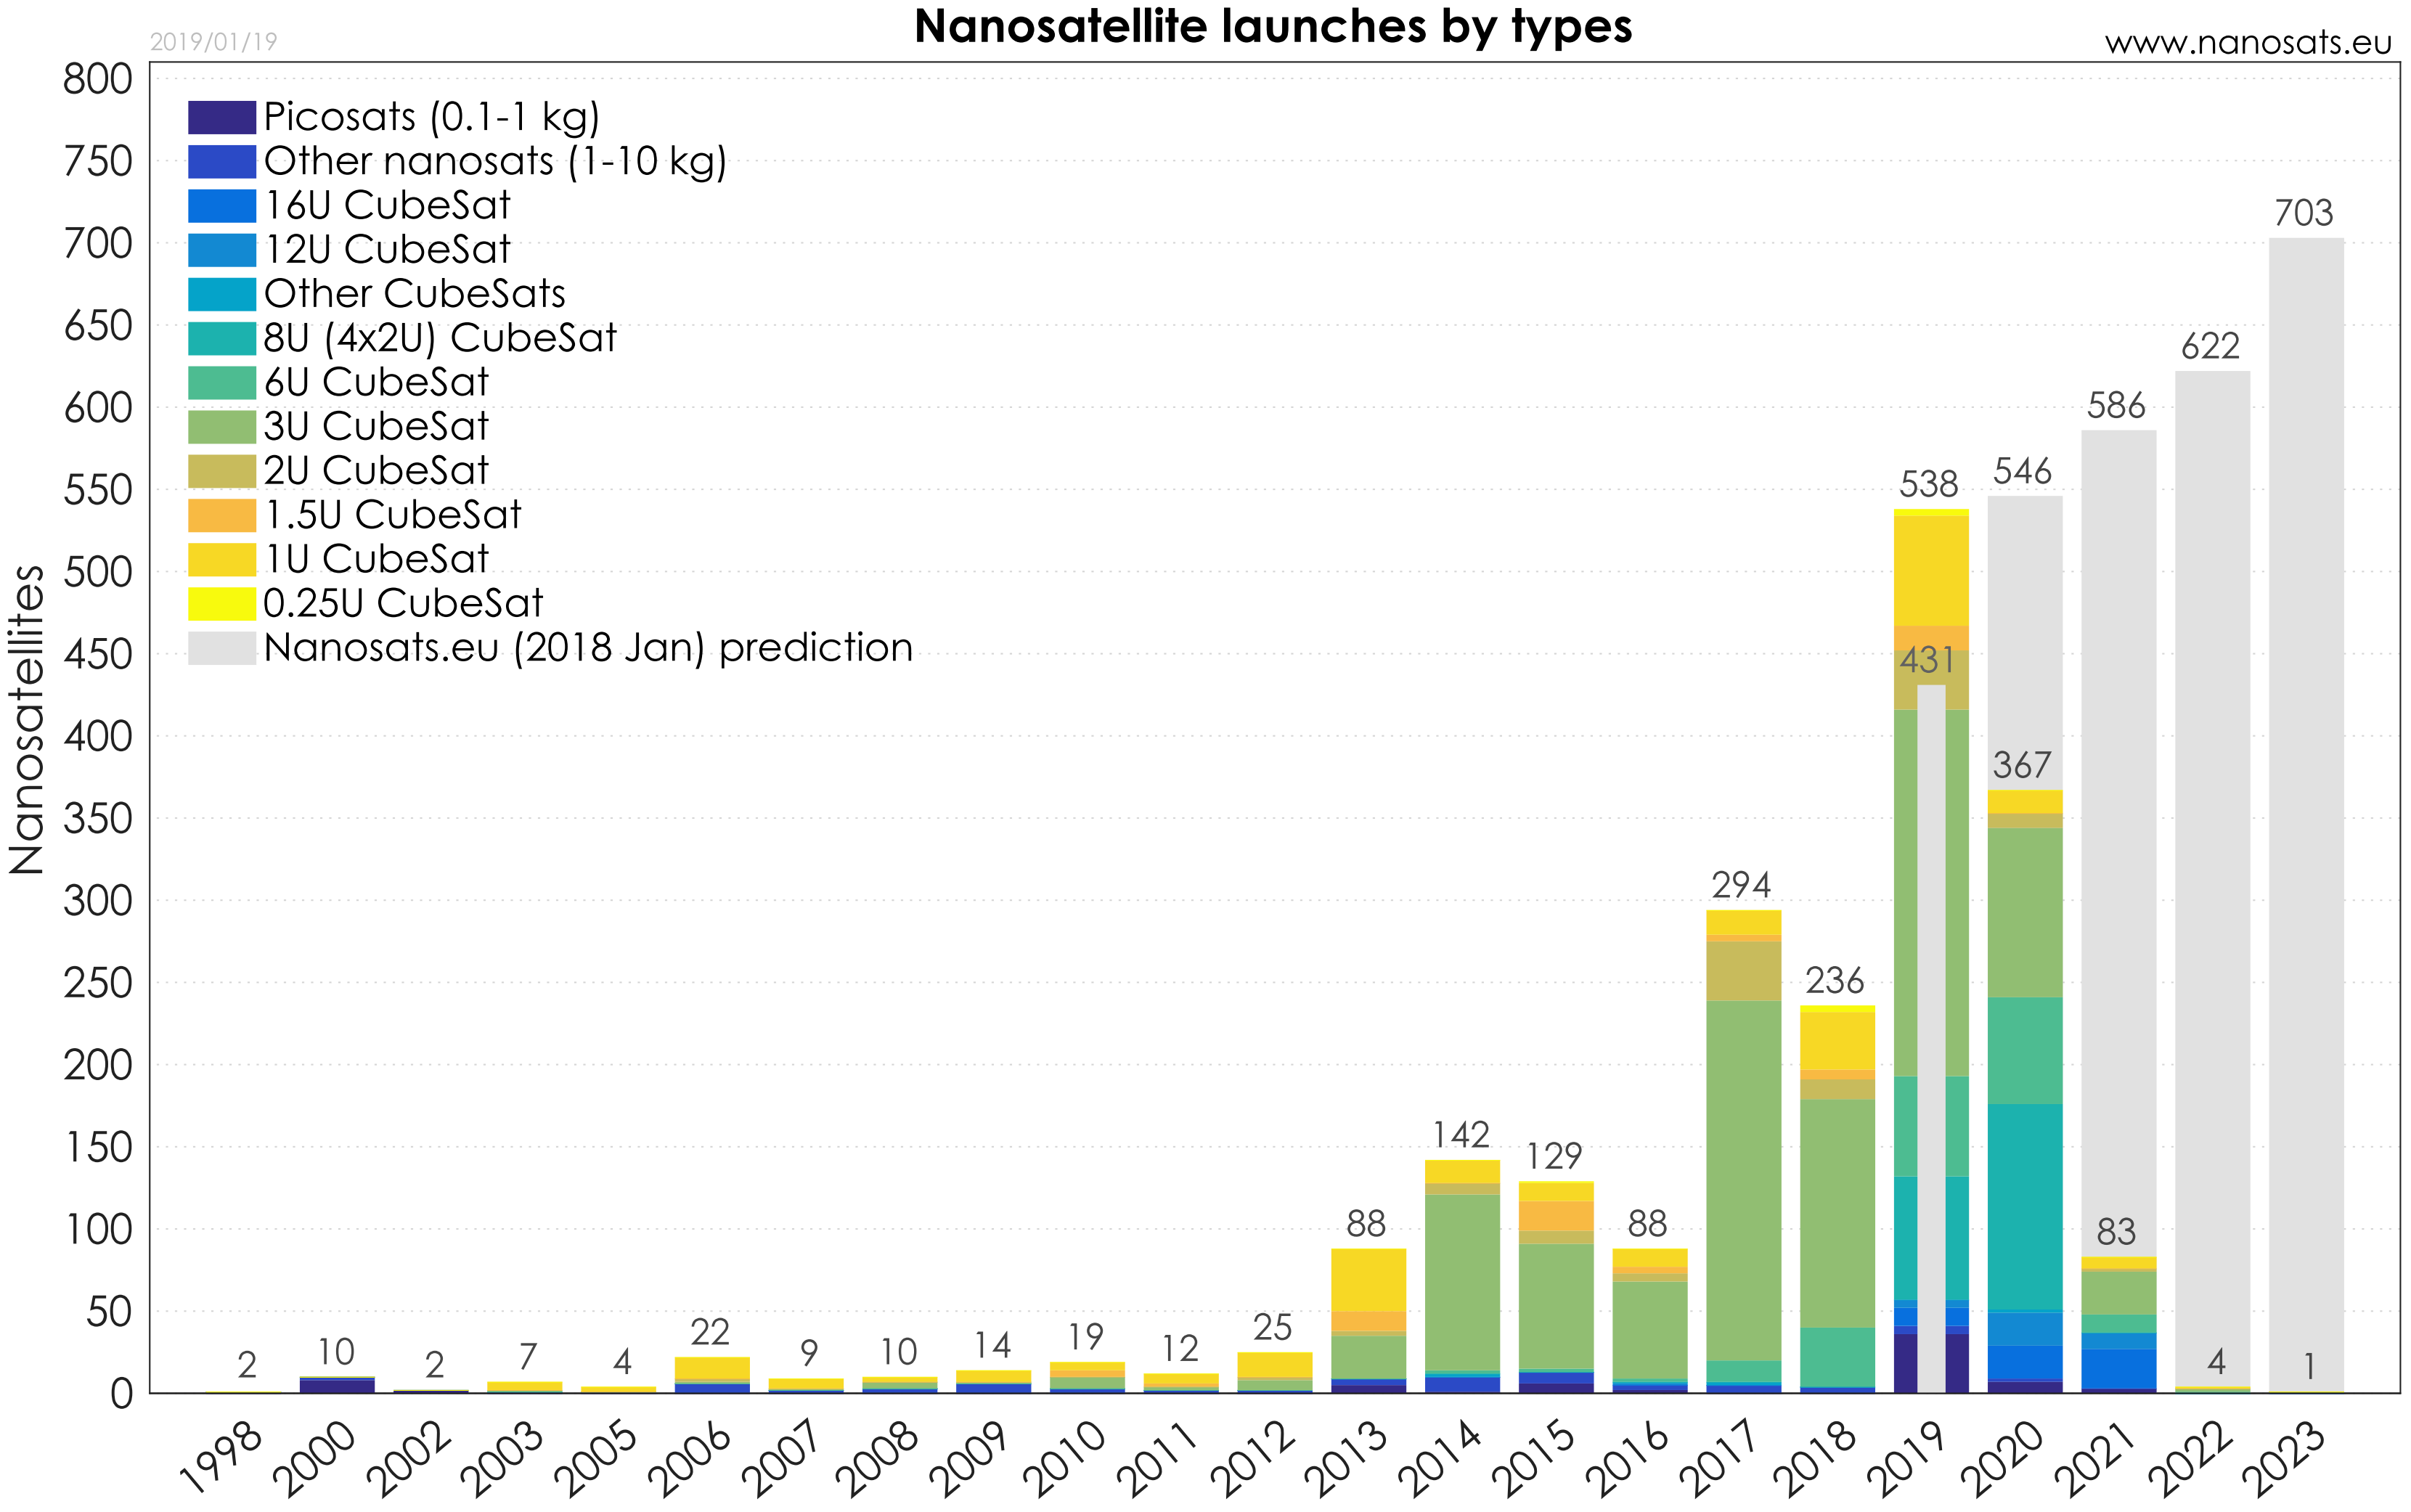
\includegraphics[width=0.80\textwidth]{Nanosats_years_types_2019-01-19_01}
				\caption{Überblick über Nanosatelliten Missionen von 1998 bis 2023}
				\label{fig:NanosatsTypes}
			\end{figure}

	\newpage
	%------------------------------------------------------------------------------------------------------------------------------------------------------------------------------
	\subsection{Gestaltungsrichtlinien}%-------------------------------------------------------------------------------------------------------------------------------------------
Für die Gestaltung von CubeSats gelten eine Reihe von Richtlinien. Als kleinste Einheit (1U) wird ein Würfel mit einer Kantenlänge von 10cm und einer zulässigen Masse von maximal 1,33 kg vorgegeben. Für größere Volumen und Massen können mehrere Einheiten von CubeSats verbunden werden. Satelliten mit 1U, 1.5U, 2U, oder 3U können von dem einheitlichen Startmechanismus (P-Pod) in die Erdumlaufbahn ausgelassen werden. Die Kosten von CubeSat Missionen können gering gehalten werden, indem diese als sekundäre Nutzlast bei Raketenstarts mitfliegen. Für größere Satelliten (6U, 12U, 27U) werden andere Startmechanismen benötigt. Die zugelassene Masse wird auf 2 kg/U angehoben. Weitere Vorschriften gelten für die Folgenden Kriterien:
		\begin{itemize}
			\item \textit{Materialien:} 	\\ Alle bei der Konstruktion verwendeten Materialien müssen den Richtlinien der Air Force Space Command Manual\cite{AFspacemanual} entsprechen. Außerdem darf der Masseverlust des Satelliten maximal 1\% betragen.
			\item \textit{Energiespeicher:} \\ Der chemische Energiespeicher darf eine Größe von 100 Wh nicht überschreiten. 
			\item \textit{Aktivierungszeitpunkt:} \\ Während der CubeSat im P-POD verstaut ist müssen alle Systeme ausgeschaltet bleiben. Beim Verlassen der Trägerrakete wird der Satellit aktiviert. Erst 30 Minuten später dürfen Bauteile (z.B. Solarpanele, Antennen, etc...) ausgefahren werden. Bevor die ersten Signale generiert oder gesendet werden müssen mindestens 45 Minuten vergangen sein. 
		\end{itemize}
Falls ein Entwurf nicht den Vorschriften entspricht, kann bei dem Betreiber der Trägerrakete eine Sondergenehmigung angefragt werden. Nach einer Reihe von Tests entscheidet dieser ob er die Abweichungen akzeptiert, Änderungen vorgenommen werden müssen, oder ein anderer Anbieter gefunden werden muss. 

%-----------------------------------------------------------------------------------------------------------------------------------------------------------------------------
	\section{Cubesat Subsysteme}%-------------------------------------------------------------------------------------------------------------------------------------------
	%hier Hauptsächlich das Fazit von max kompakt darstellen und refernzieren
		\subsection{Antrieb}%----------------------------------------------------------------------------------------------------------------------------------------------------
Eines der wichtigsten Subsysteme für Active Debris Removal (ADR) Missionen mit einem CubeSat ist der Antrieb. Er wird für Lageregelung und das Deorbiting des Zielobjekts benötigt.
Für CubeSats stehen nur wenige ausgereifte und erprobte Triebwerke zur Verfügung [Literatur].  Die Miniaturisierung bestehender Technologien stellt eine große Herausforderung dar. Ein hoher TRL ist für die Auswahl besonders Entscheidend, da nur bereits erprobte Technologien für diese Mission genutzt werden sollten.
Im Wesentlichen lassen sich die Antriebsarten in chemische und elektrische Antriebe unterteilen.  Chemische Antriebe generieren im Allgemeinen einen höheren Schub und werden für impulsive Manöver verwendet. Für den Betrieb muss ein großer Gewichtsanteil an Treibstoff einkalkuliert werden. Der spezifische Impuls ist jedoch deutlich niedriger als bei elektrischen Antrieben. Diese bieten auch ein besseres Schub-Leistungs-Verhältnis. Elektrische Antriebe sind jedoch auf eine ausreichende externe Energiequelle angewiesen. Diese wird zwangsläufig benötigt, um die getankte Masse zu beschleunigen [Literatur].
Für genaue Untersuchung und den Vergleich der verschiedenen Triebwerkstypen wird auf [Literatur] verwiesen. Miniaturisierte Versionen von erprobten Triebwerken werden stetig weiterentwickelt und getestet. Es wurden bereits mehrere Miniaturisierte Triebwerke in CubeSatmissionen erfolgreich eingesetzt. In Zukunft sollte es eine wachsende Auswahl an geeigneten Triebwerken für CubeSat-Missionen geben. 
Eines der wichtigsten Subsysteme für Active Debris Removal (ADR) Missionen mit einem CubeSat ist der Antrieb. Er wird das Deorbiting des Zielobjekts benötigt.  Um Lageregelung und Rendezvous-Manöver durchführen zu können müssen sehr präzise Triebwerke gewählt werden. Für CubeSats stehen nur wenige ausgereifte und erprobte Triebwerke zur Verfügung unter anderem durch die Herausforderung der Miniaturisierung bestehender Technologien.  
Ein hoher TRL ist für die Auswahl besonders Entscheidend, da nur bereits erprobte Technologien für diese Mission genutzt werden sollten.
Im Wesentlichen lassen sich die Antriebsarten in chemische und elektrische Antriebe unterteilen.  Chemische Antriebe generieren allgemein einen höheren Schub und werden für impulsive Manöver verwendet. Für den Betrieb muss ein großer Gewichtsanteil an Treibstoff einkalkuliert werden. Der spezifische Impuls ist jedoch deutlich niedriger als bei elektrischen Antrieben. Diese bieten auch ein besseres Schub-Leistungs-Verhältnis. Elektrische Antriebe sind jedoch auf eine größere externe Energiequelle angewiesen. Diese wird zwangsläufig benötigt, um die getankte Masse zu beschleunigen. \cite{Lettau.}
Für genaue Untersuchung und den Vergleich der verschiedenen Triebwerkstypen wird auf \cite{Lettau.} verwiesen. Miniaturisierte Versionen von erprobten Triebwerken werden stetig weiterentwickelt und getestet. Es wurden bereits mehrere Miniaturisierte Triebwerke in CubeSat Missionen erfolgreich eingesetzt. In Zukunft sollte es eine wachsende Auswahl an geeigneten Triebwerken für CubeSat Missionen geben. 

%-----------------------------------------------------------------------------------------------------------------------------------------------------------------------------------
		\subsection{Stromversorgungssystem - Electrical Power System (EPS)}%----------------------------------------------------------------------------------------------------
Das EPS ist für die Erzeugung-, Speicherung- und Verteilung von elektrischer Energie verantwortlich. 
Für die Stromerzeugung werden in der Raumfahrt hauptsächlich Solarpanele verwendet, welche auch für CubeSats die sinnvollste Lösung darstellen.
Für die meisten Anwendungen können Produkte verschiedener Anbieter COTS erworben werden. CubeSats mit geringem Leistungsbedarf nutzen oft nur ihre eigene Oberfläche um mit Solarzellen Strom zu generieren. Wenn mehr Leistung benötigt wird werden faltbare Solarmodule genutzt. So kann die nutzbare Oberfläche zwei bis vier mal größer sein, als die benötigte Fläche auf dem Satelliten.\cite{Lettau.}\\
Während der Satellit sich im Schatten der Erde befindet wird Energie aus einem internen Speicher genutzt. Dieser besteht in der Regel aus Lithium basierten Akkus, welche eine hohe Energiedichte von bis zu 240 Wh/kg aufweisen. Sie können sowohl als einzelne Zellen, als auch in vorgefertigten Paketen COTS erworben werden.\cite{Lettau., Abaker.2017}\\
\begin{figure}[!h]
	\centering
		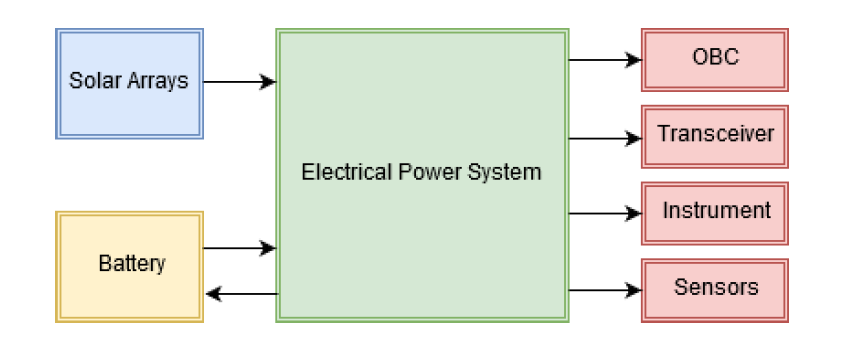
\includegraphics[width=0.50\textwidth]{./graphics/Struktur_EPS.PNG}
	\caption{EPS Aufbau \cite{Pelgrift.2017}}
\end{figure}
\newpage

	Für die Verteilung des Stroms an die Subsysteme gibt es zwei unterschiedliche Ansätze. Zum Einen sind es dezentralisierte Verteilungssysteme, die ein modulares und flexibles Design erlauben. Dieses kann für verschiedene Satelliten angepasst werden. Es arbeitet mit nur einer Ausgangsspannung, die dann für jedes angeschlossene Subsystem einzeln umgewandelt wird.\\
\begin{figure}[!h]
	\centering
		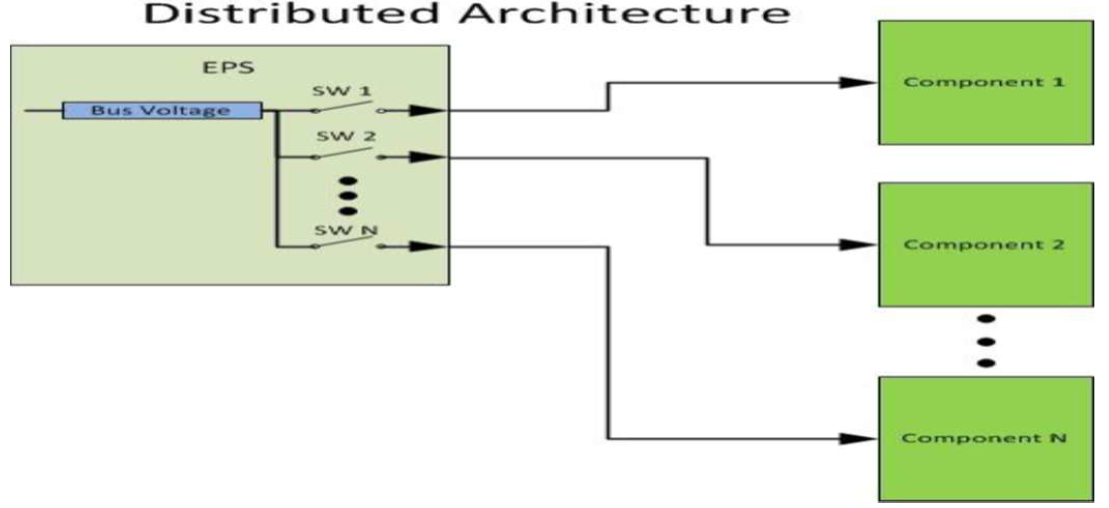
\includegraphics[width=0.50\textwidth]{./graphics/Distributed_EPS.PNG}
	\caption{Dezentralisiertes EPS \cite{Abaker.2017}}
\end{figure}

 Die zweite Variante sind zentralisierte Verteilungssysteme. Diese werden häufiger verwendet, da sie den Vorteil eines geringen Volumens bieten und weniger Spannungsregler benötigen. Das wird erreicht, indem alle Subsysteme mit gleicher Spannung am selben Regler angeschlossen werden. Nachteilig ist, dass dieser Regler auf die maximale Gesamtlast aller Subsysteme ausgelegt werden muss. Das führt dazu, dass zentralisierte Systeme zwar im Aufbau einfacher ausfallen, jedoch aufgrund der Maximallastauslegung weniger effizient sind.\cite{Abaker.2017}
\begin{figure}[!h]
	\centering
		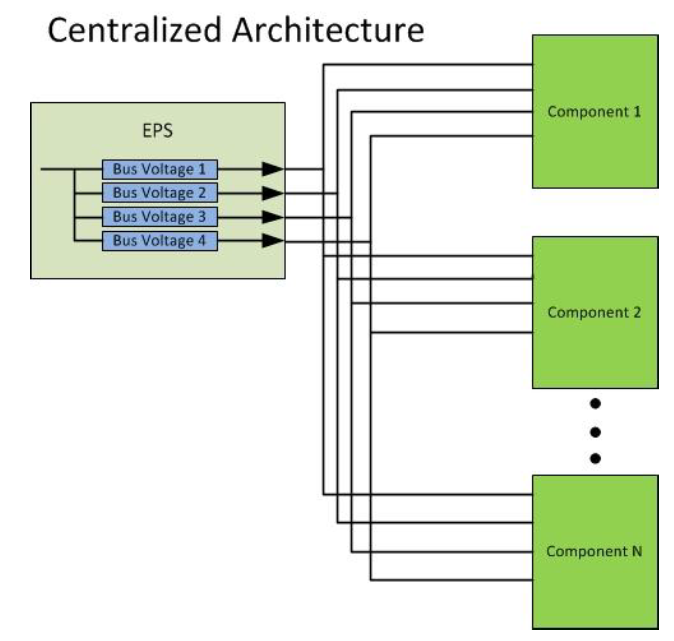
\includegraphics[width=0.50\textwidth]{./graphics/Centralized_EPS.PNG}
	\caption{Zentralisiertes EPS \cite{Abaker.2017}}
\end{figure}




		%-----------------------------------------------------------------------------------------------------------------------------------------------------------------------------
		\subsection{Guidance, navigation and control -GNC ADCS}%------------------------------------------------------------------------------------------------------------------
		Guidance, Navigation and Control (GNC) Subsysteme sind neben den in Kapitel [...] genannten Systemen unabdingbar für ADR Missionen, da diese die Positionsbestimmung als auch die Lagebestimmung und Regelung beinhaltet. Dieses System kann in zwei Hauptbereiche unterteilt werden: der Lage- und Positionsbestimmung, sowie der Lageregelung.
Bei der Lage und Positionsbestimmung kann auf verschiedene Sensoren zurückgegriffen werden. Die absolute Positionsbestimmung erfolgt über eine Bodenstation, welche auch zur Kommunikation mit dem Satelliten verwendet wird. Bei dieser Art der Positionsbestimmung ist es notwendig zu wissen, welchen geplante Erdumlaufbahn der Satellit hat. Diese Methode bezieht sich auf der Zeitdifferenz zwischen Sende- und Empfangszeitpunkt. Deswegen ist die Positionsbestimmung via Bodenradar nicht sehr genau[quelle]. Seit der erfolgreichen Miniaturisierung  von GPS Empfängern werden auch diese zur Positionsbestimmung verwendet. Dies funktioniert solange die GPS Satelliten die Einsatzhöhe von CubeSats überschreiten. Die Lagebestimmung über Startracker erfolgt in dem ein Bild des Himmels mit einem Katalog abgeglichen wird.. Dadurch kann die Lage bei bekannter Position bestimmt werden. Weitere Möglichkeiten sind Sonnen-, Erd- Magnetfeldsensoren, sowie Kreiselinsturmente. Bei Kreiseln wird die Verdrehung im Vergleich zu einem aufgeprägten Inertialsystem gemessen, wodurch die Lage genau bestimmt werden kann. 
Die Regelung  der Lage kann über unterschiedliche Methoden erfolgen. Die einfachste ist eine Drehbewegung um eine der Hauptachsen. Dies führt zu einer Stabilisierung des Satelliten, ist jedoch für eine CubeSat, dessen Aufgabe das Docking und deorbiting beinhaltet, nicht sinnvoll. Dementsprechend kann eine 3 achs-Stabilisierung durchgeführt werden, welche durch Triebwerke und Reaktionsräder durchgeführt werden kann. Diese Art der Lageregelung benötigt ein Reaction Control System (RCS) um unkontrollierte bewegungen zu vermeiden. Die Regelung mittels RCS-Triebwerken geschieht indem Schubimpulse in die jeweilige Richtung gegeben werden. An allen drei Hauptachsen sind Schwungräder montiert. Durch den Antrieb der Räder wird ein Moment erzeugt welches den Satelliten in die gewünschte Lage bringt. Da ein 3-achs System nicht nur Stabilisiert, sondern auch die gewünschte Lage herbeiführen kann, ist dieses System für den viele Fälle optimal.

%------------------------------------------------------------------------------------------------------------------------------------------------------------------------------
		\subsection{Command and data handling}%-------------------------------------------------------------------------------------------------------------------------------------
		Das Command- und Data-handling Subsystem (CDHS) ist die Prozessoreinheit, die sich um alles kümmert was mit Software gesteuert wird. Hier werden Daten zu allen Subsystemen und Nutzlasten gesammelt. Das CDHS stellt die Daten bereit, die übertragen werden sollen und führt Befehle aus, die an das Kommunikations Subsystem gesendet werden. 
Es sorgt für die korrekte Einstellung der Solarzellen und Ladung der Batterien. Alle Berechnungen zur Position in der Erdumlaufbahn und der aktuellen Zeit finden hier statt.
Neben dem aktiven Ausführen von Befehlen beobachtet und löst der Prozessor eine Reihe an Problemen, die während der Mission auftreten können.
Die Bestandteile des CDHS sind der Raumflugrechner, die Flugsoftware und ein Speichermedium.

%--------------------------------------------------------------------------------------------------------------------------------------------------------------------------------
		\subsection{Kommunikation}%-----------------------------------------------------------------------------------------------------------------------------------------------
		Das Kommunikations Subsystem sorgt bestenfalls für eine dauerhafte Verbindung zur Bodenstation. Aufgezeichnete Daten und eingehende Befehle werden hier von, und an den Cubesat übertragen. Das Subsystem besteht aus den Telemetrie- und Befehlsystemen.
Das Telemetriesystem besteht aus einem oder mehreren Transmittern, welche die vom Prozessor kommenden Daten als Signal an die Bodenstation über die Antennen an Bord des Cubesats aussenden. Die Signale werden als Mikrowelle übertragen und empfangen. Je nach verwendetem System handelt es sich dabei um S-Band-, oder X-Band Wellen. Wellen im X-Band Spektrum können zwar, aufgrund der höheren Frequenz, höhere Bandbreiten erreichen, aber die Technologie ist noch nicht so etabliert wie S-Band Transmitter.
		
		%---------------------------------------------------------------------------------------------------------------------------------------------------------------------------
		\subsection{Thermik}%------------------------------------------------------------------------------------------------------------------------------------------------------
Die Wärme wird im Vakuum durch Strahlungen und Wärmeleitungen übertragen. Das Wärmemanagement regelt den Bereich der zulässigen Temperaturen für die Sicherstellung einer optimalen Funktionalität und das Überleben des Satelliten. Durch die Massen-, Volumen- und Leistungsbeschränkungen bei miniaturisierten Satelliten, wie dem CubeSat, liegt der Fokus auf den passiven Wärmereglungstechnologien, da die Fortschritte bei der Entwicklung von miniaturisierten aktiven Wärmeregelungsmethoden begrenzt ist. Passive Technologien sind mit geringen Kosten, Volumen, Gewicht und Risiko verbunden und erfordern keine interne Eingangsleistung für die Wärmeregulierung. Thermische Beschichtungen, Wärmerohre, Sonnenschirme, Wärmebänder und Multi-Layer Insulation (MLI) sind passive Methoden für die Regulierung des thermischen Gleichgewichtes. Die aktiven Methoden, wie elektrische Widerstandsheizungen, Kühler oder kryogene Materialien, sind mit höherer Präzision und interner Eigenleistung verbunden. Die Verwendung von aktiven Systemen ist bei temperaturempfindlichen Geräten und nicht ausreichender, passiver Systeme für eine Aufrechterhaltung der Betriebstemperatur vielversprechender. \cite[S. 109 - 120]{NASA.Sota.2018} 

%------------------------------------------------------------------------------------------------------------------------------------------------------------------------------
		\subsection{Struktur}%-------------------------------------------------------------------------------------------------------------------------------------------
Die Strukturen werden in Primär- und Sekundärestrukturen unterteilt. Die Primärstruktur ist thermischen und dynamischen Beeinflussungen ausgesetzt, denen sie entgegenwirken muss. Des Weiteren sorgt es für Lastübertragung während des Starts und des Einsatzes. Elektromagnetische Strahlungen, Drücke und innere Wärmeleitungen sind weitere Faktoren die einen großen Einfluss auf das Gehäuse haben und deshalb mit einbezogen werden müssen. Die Begrenzungen bei der Oberfläche und bei dem Volumen sorgen für Einschränkungen. Infolgedessen sollte sie effizient ausgelegt werden. Komponenten die nur sich selbst tragen müssen, wie Sonnenkollektoren, zählen zu den Sekundärstrukturen auf die nicht näher eingegangen wird, da sie bei einem Ausfall die Integrität des Raumfahrzeugs nicht beeinträchtigt. Die Primärstrukturen werden als COTS-Strukturen und kundenspezifisch bearbeitet oder gedruckte Komponenten auf dem Markt angeboten. Generell besteht das Gehäuse aus metallischen und nichtmetallischen Materialien und wird von der Betriebsumgebung des Satelliten bestimmt. \cite[S. 96 - 108]{NASA.Sota.2018} 

%------------------------------------------------------------------------------------------------------------------------------		
	\section{ADR Methoden}
%------------------------------------------------------------------------------------------------------------------------------	
Für eine ADR Mission gibt es verschieden Methoden um diese durchzuführen. Die Grafik zeigt unterschiedliche Cluster von ADR Methoden, welche unterschiedliche Vor-und Nachteile, sowie TRL haben. Im Folgenden wird auf jedes Cluster eingegangen, beschrieben und den aktuellen Status erläutert.
	
				\begin{figure}[h]
				\centering
					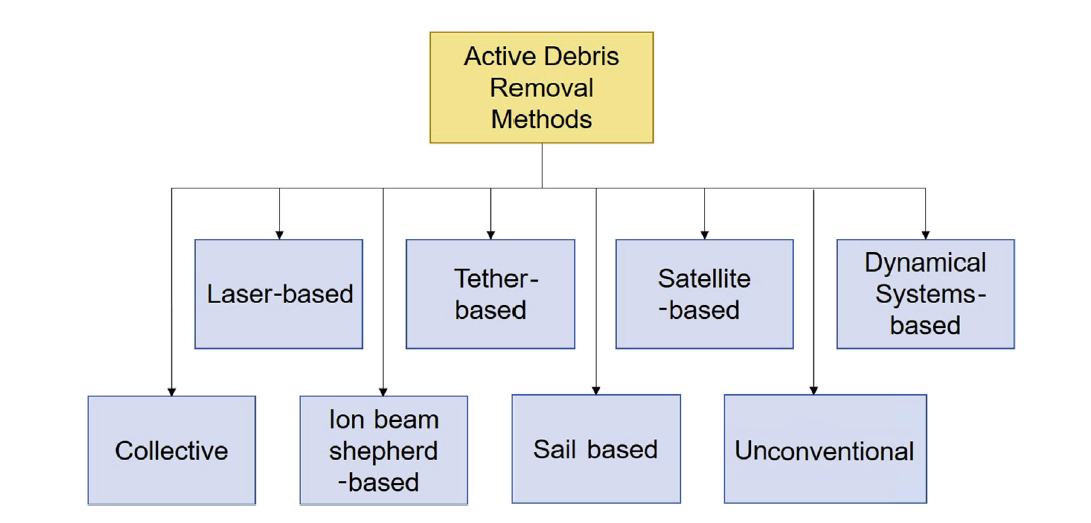
\includegraphics[width=0.80\textwidth]{./graphics/ADR/ADR_methods.PNG}
				\caption{Überblick über die ADR Methoden}
				\label{fig:ARD Methoden}
			\end{figure}
Es gibt einige Herausforderungen, welch unabhängig von der Removal Methode sind und für jede Mission individuell gelöst werden muss. Dazu gehört die Klassifizierung der zu entfernenden Objekte, sowie dessen genaue Positionsanalyse. Sollen während einer Mission mehrere Objekte entfernt werden, so muss zu beginn definiert werden in welcher Reihenfolge dies geschehen soll. 

%---------------------------------------------------------------------------------------------------------------------
	\subsection{Collective Method}
%----------------------------------------------------------------------------------------------------------------------	
	
				\begin{figure}[h]
			\centering
					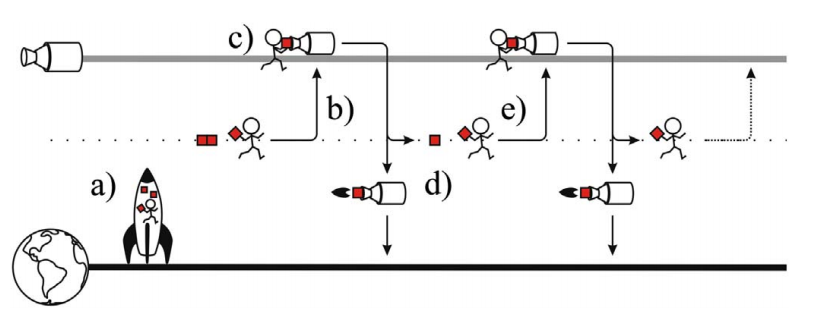
\includegraphics[width=0.80\textwidth]{./graphics/ADR/collective_method.PNG}
				\caption{Missionsaufbau für Collective Method}
				\label{fig:Sammelmethoden}
			\end{figure}
	
Die Abbildung zeigt den grundlegenden aufbau eine ADR mission welche auf einer kollektiven Methode beruht. Dabei wird ein Satellit mit Deorbiting Kits ausgestattet, welcher die verschieden Ziele anfliegt und diese anbringt. Ein großer Vorteil ist, dass nur ein Trägersatellit mit anspruchsvoller Technik für die Navigation, Positionsbestimmung , Dockingmechnismen und Energieversorgung ausgestattet werden muss. Da der Trägersatellit mehrer Ziele anfliegt, muss dieser über ein sehr großes Tankvolumen verfügen, da mehrer Orbithöhe anhebungen durchgeführt werden müssen. Neben der Orbithöhe muss vermutlich auch eine änderung der Inklination und exzentrizität durchgeführt werden. Dies kann auch bei kleinen Unterschieden der Variablen zu einem sehr hohen Treibstoffverbrauch führen. Außerdem wird bei jedem Zielobjekt ein Rendezvous Manöver sowie docking durchgeführt, welche das Potential haben durch eine Kollision weiter Trümmer zu erzeugen. Aktuell wird an der Validierung dieser Methode anf der Erde geforscht.

%------------------------------------------------------------------------------------------------------------------------
			\subsection{Laser-based Method}
%-----------------------------------------------------------------------------------------------------------------------
Wie der Name es bereit sagt beruht diese Methode auf Laser , welcher sich auf der Erde befindet. Es wird ein hochenergetischer Laser benötigt, welcher in einer geringen Zeit das Objekt befeuert. dadurch entsteht ein Plasmastrahl, welcher den Satelliten bremst und dadurch eine Verringerung der Orbithöhe resultiert. Dieses System kann dazu verwendet werden um sowohl große als auch kleine Objekte zu entfernen, sowie dessen kosteneffizient. Das größte Problem bei dieser Methode, ist die Zielfindung und Verfolgung. Damit das deorbiting funktioniert muss der Laser für ein bestimmtes Zeitinkrement auf das Ziel gerichtet sein, was eine genau Berechnung der Zielposition in Abhängigkeit der Dauer von Start des Laserstrahls und erreichen des Ziels.
	
	\begin{figure}[h]
			\centering
					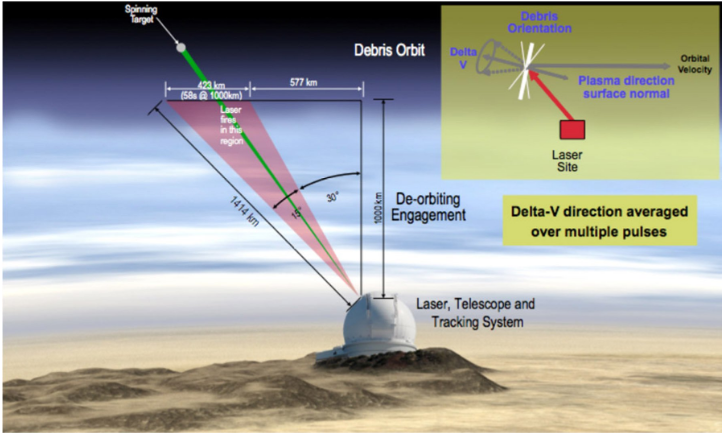
\includegraphics[width=0.80\textwidth]{./graphics/ADR/Laser-beam.PNG}
				\caption{Funktionsweise des ADR mittels Laser}
				\label{fig:Laser}
			\end{figure}

%-------------------------------------------------------------------------------------------------------------------------
\subsection{Ion beam shepherd-based Method}

	\begin{figure}[h]
			\centering
					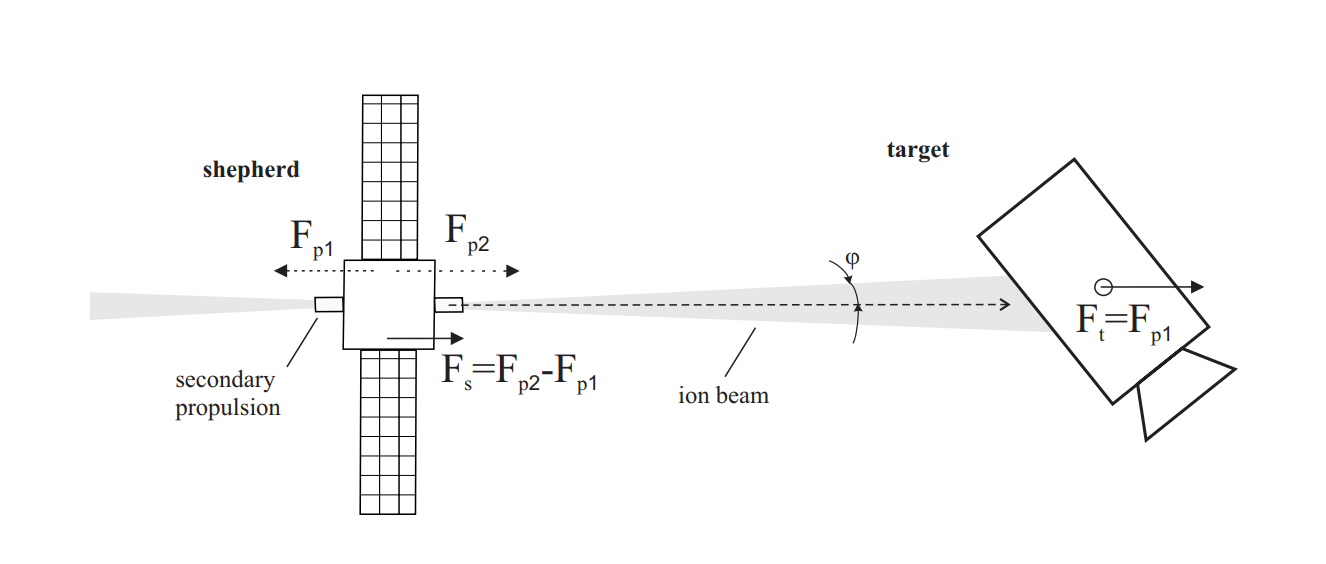
\includegraphics[width=0.80\textwidth]{./graphics/ADR/Shepherd.PNG}
				\caption{Funktionsweise des ADR mittels Laser}
				\label{fig:Laser}
			\end{figure}

Die Abbildung  zeigt den schematischen Aufbau einer ADR Mission nach Ion Based Shepherd Methode. Der Chaser Fliegt vor dem Zielobjekt und bremst diesen durch ein Ionenstrahl aus dem zum Objekt gerichteten Triebwerk. Besonders zu beachten ist die Streuung des Ionenstrahl und die genaue Positionierung des Chasers vor dem Zielobjekt.

%------------------------------------------------------------------------------------------------------------------------------		
	\section{RDVDO Mechanismen} das kann ausführlich sein
%------------------------------------------------------------------------------------------------------------------------------	
		\subsection{Docking Strategien}
						\textbf{Roboterarm}
						\textbf{Fangnetz}
						\textbf{Adhäsiv Docken}
						%Übersichtstabelle/Graphik: sihe die Quellen die ich am 15.05.2019 gezeigt habe
		\newpage
		
	%------------------------------------------------------------------------------------------------------------------------------------------------------------------------------
		\subsection{Bionische Materialien}%-------------------------------------------------------------------------------------------------------------------------------------------
Gecko-inspirierte mikrostrukturierte Oberflächen scheinen eine vielversprechende Lösung für das Dockingproblem bei ADR Missionen zu sein. Mittels trockener Adhäsion können Geckos in der Natur an Oberflächen haften. Durch die hierarchische Struktur ihrer Füße entstehen Van-der-Waals-Wechselwirkungen. Die kleinsten Fasern haben einen Durchmesser und eine Länge von einigen Nanometern. Insgesamt besitzt ein Gecko über 500000 Hafthaare an einem Fuß. Sie bilden eine Flexible Struktur, die problemlos an glatten oder rauen Oberflächen haftet. Da für das Docking etwas genutzt werden muss, das den Bedingungen im Weltraum wie Vakuum, Strahlung und Kälte standhält, sollen Geckomaterialien für diese Anwendung näher untersucht werden. Besonders vorteilhaft ist das zerstörungsfreie Andocken mittels der Geckostruktur, was das Risiko neu entstehender Trümmerteile verringert.
Van-der-Waals-Wechselwirkungen sind grundlegend molekulare Wechselwirkungen. Indem temporäre Umverteilungen von Elektronen in einem Molekül stattfinden entstehen Bereiche die unterschiedlich geladen sind (Dipole). Diese haben Auswirkungen auf benachbarte Moleküle. Es entsteht eine Kettenreaktion von Dipolbildungen, die zu Anziehungskräften zwischen Positiv und Negativ geladenen Bereichen naher Moleküle führt. Jedes Kleinsthaar baut dabei eine Haftkraft auf. Mit einer steigenden Anzahl an Bindungsstellen erhöht sich auch die gesamte Haftkraft. Außerdem wird die Ablösekraft größer, desto kleiner die Strukturdurchmesser sind, da auf einer kleinen Fläche eine Vielzahl an Kontakten entstehen. \cite{Schwerter.}
Mit dem heutigen Stand der Technik ist es möglich diese Mikrostrukturen kostengünstig und schnell mit bestimmten Verfahren reproduzierbar herzustellen. Diese synthetisch hergestellten Mikrostrukturen erreichen bereits ähnliche Haftkräfte wie ihre natürlichen Vorbilder. Mit den Strukturen aus \abb{fig:Gecko1} wurden Haftkräfte von 10 $\frac{N}{mm^{2}}$ und Scherbeanspruchungen (Ablösekräfte)  von 2 $\frac{N}{mm^{2}}$ gemessen.
	\begin{figure}[h]
	\centering
		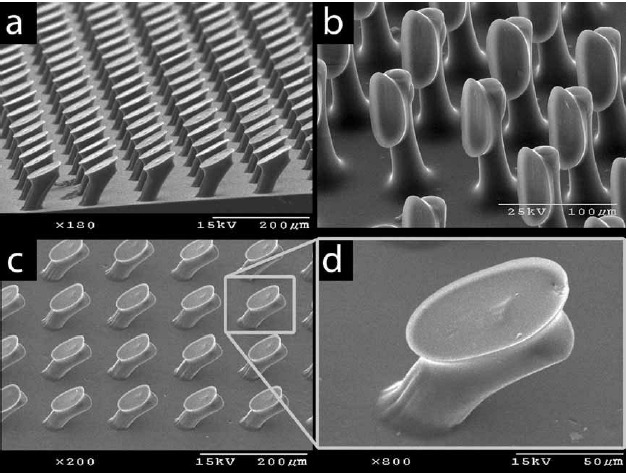
\includegraphics[width=0.70\textwidth]{Gecko1}
	\caption{Aufnahme einer Mikrostruktur mit 35 $\mu m$ Durchmesser. Strukturen weisen unterschiedliche Winkel auf: a) 	34\textdegree{}  b) 90\textdegree{}  c),d) 23\textdegree{} \cite{Schwerter.} \cite{Schwerter.}}
	\label{fig:Gecko1}
\end{figure}
Eine genaue Auflistung der erreichten Haftkräfte für die verschiedenen Ausführungen der Mikrostruktur und Belastungsfälle ist in \cite[Tabelle1, Seite 23]{Schwerter.} zu finden.
Polydimethylsiloxan (PDMS) Strukturen erreichen maximale Scherkräfte in Haftrichtung von 34,8 $\frac{N}{mm^{2}}$ und einer Normalkraft von 10,8 $\frac{N}{mm^{2}}$.
PDMS Strukturen wurden bereits erfolgreich in der Schwerelosigkeit getestet. Diese konnten an einem Greifer verschiedene Objekte einfangen und bewegen \cite{Schwerter.}. Außerdem wurde durch mehrere Versuchsreihen nachgewiesen, dass Temperatur und Vakuum kaum einen Einfluss auf die Leistungsdaten haben. Verschiedene Mikrostrukturen wurden einer thermischen Wechselbeanspruchung zwischen 125 und  -125 \textdegree{} C unterzogen und daraufhin in Vakuum und Normalbedingungen getestet. Durch die Temperatur ist kein Einfluss zu verzeichnen. Das Vakuum ruft nur vernachlässigbare Änderungen in Vorspannung und Haftung hervor \cite[Seite 7, Figure 11]{Moreels.}. Durch Tests mit verschiedenen Materialien konnte festgestellt werden, dass die Oberfläche, an der die Struktur haften soll einen relativ geringen Einfluss auf die Haftung hat \cite[Seite 9, Figure 16]{Moreels.}. 

Bei der technischen Anwendung ist zu beachten, dass es eine Haftrichtung und eine Ablöserichtung in der Struktur gibt. Die haltbaren Scherkräfte in Ablöserichtung sind somit um bis zu Faktor 10 geringer als in Haftrichtung\cite{Schwerter.}.
\begin{figure}[h]
	\centering
		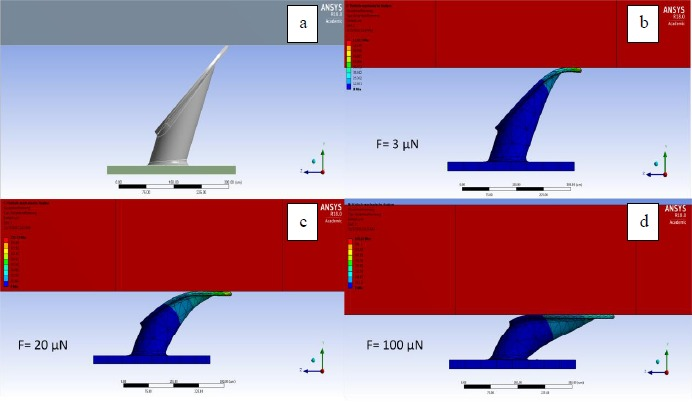
\includegraphics[width=0.70\textwidth]{Gecko2}
	\caption{Simulation des Verformungsverhaltens der Mikrostruktur bei Haftberührung \cite[Abbildung 19, Seite43]{Schwerter.}}
	\label{fig:Gecko2}
\end{figure}	


In der Simulation (\abb{fig:Gecko2}) ist gut zu erkennen, dass die Mikrosäulen mit dem Haftprofil in eine vorbestimmte Richtung belastet werden sollen. Andernfalls können sie nicht die maximale Haftfläche nutzen und es geht Haftkraft verloren [Literatur, Abb.26 u. ff]. 
Allgemein wird eine Steigerung der Normalkraft und der Scherkräfte durch Erhöhung der Anpresskraft festgestellt. Optimaler Halt sollte also mit einer Vorspannkraft, die beim anbringen der Mikrostruktur ausgeübt wird erreicht werden [Literatur].  Zukünftig besteht die Möglichkeit verschiedene Formen der Hafthaare zu kombinieren, um deren Vorteile zu nutzen. 
Es existiert bereits ein Andockmechanismus ( \abb{fig:Gecko3}) dessen Gecko-Mikrostruktur nach  European Cooperation for Space Standardization (ECSS) Standards getestet wurde \cite[Seite 10]{Moreels.}. 


\begin{figure}[h]
	\centering
		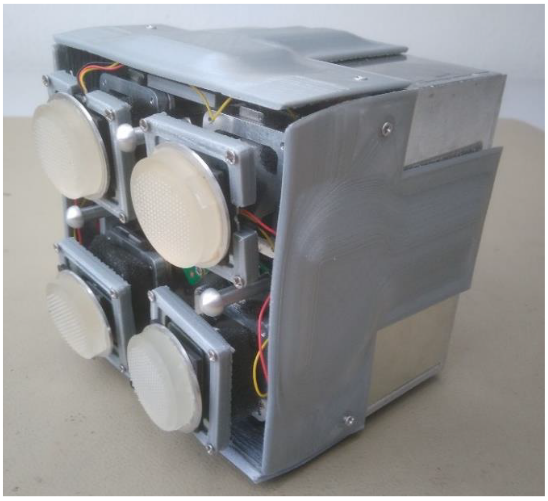
\includegraphics[width=0.50\textwidth]{graphics/Gecko3.PNG}
	\caption{Prototyp Gecko Dochingmechanismus \cite[Figure 18, Seite 10]{Moreels.}}
	\label{fig:Gecko3}
\end{figure}


Durch einen Versteifungsmodus und die aktive Lastverteilung wird eine möglichst gute Verteilung der herrschenden Kräfte erzielt \cite{ChristopherTrentlage.2018}.
Für die folgende Abschätzung der maximal wirkenden Kräfte auf die Mirkohaftstruktur wurde der Aufbau des Prototypen (\abb{fig:Gecko_Rechnung1}) vorausgesetzt. Bei den Berechnungen wird von den ungünstigsten Lastfällen ausgegangen.
In \abb{fig:Gecko_Rechnung1, fig:Gecko_Rechnung2, fig:Gecko_Rechnung3} werden die der Berechnung zugrundeliegenden Annahmen gezeigt. Die belasteten Verbindungen der Mikrohaftstrukturen zum Zielobjekt werden als feste Lager A und B angenommen. Es wird davon ausgegangen, dass die Vorspannkraft beim Andocken ideal aufgebracht wurde. Außerdem bleibt die Kombination aus kritischen Normal- und Scherkräften unberücksichtigt. Der zusätzliche Anpressdruck des Haupttriebwerks wurde ebenfalls nicht berücksichtigt.

\begin{figure}[h]
	\centering
		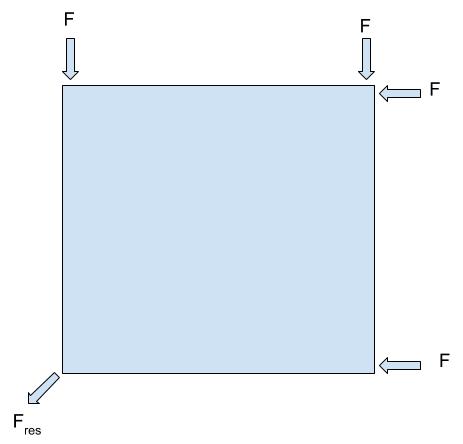
\includegraphics[width=0.50\textwidth]{graphics/Gecko_Rechnung1.png}
	\caption{Kräftebetrachtung Ansicht von oben}
	\label{fig:Gecko_Rechnung1}
\end{figure}

\begin{figure}[h]
	\centering
		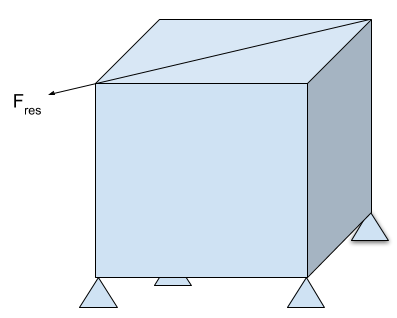
\includegraphics[width=0.50\textwidth]{graphics/Gecko_Rechnung2.png}
	\caption{Kräftebetrachtung 3D}
	\label{fig:Gecko_Rechnung2}
\end{figure}

\begin{figure}[h]
	\centering
		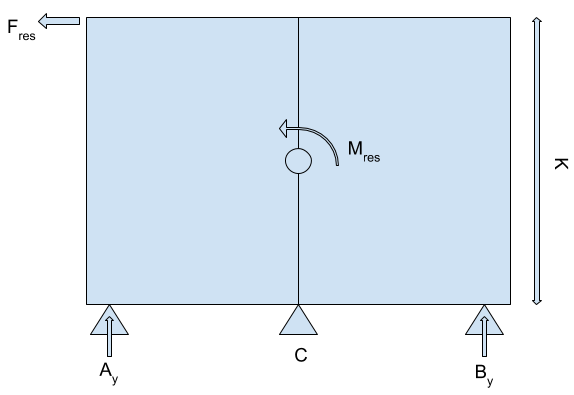
\includegraphics[width=0.50\textwidth]{graphics/Gecko_Rechnung3.png}
	\caption{Kräftebetrachtung Momentengleichgewicht}
	\label{fig:Gecko_Rechnung3}
\end{figure}


Wie in \abb{fig:Gecko_Rechnung1} und \abb{fig:Gecko_Rechnung1} zu erkennen ist Wirken bei der Maximalen Belastung durch Normalspannung vier Düsen des RCS-Systems mit einem Schub von jeweils $0,23 N$ \kap{Angenommenes Design}. Die auftretenden Kräfte werden zur resultierenden Kraft $F_{res}$  zusammengefasst:

	\begin{eqnarray}
			F_{res}=\sqrt{ 2 }*2F
	\end{eqnarray}

Über das Momentengleichgewicht lässt sich die wirkende Kraft in y-Richtung des Festlagers $B_y$  bestimmen (\abb{fig:Gecko_Rechnung3}).

\begin{eqnarray}
		\sum{  }{  }{ M_{(C)} }=0=-B_y*CB+AC*A_y+F_{res}*K
\end{eqnarray}

$B_y$ entspricht der maximalen Normalkraft, die einen Haftpunkt belasten kann. Mit einer Sicherheit von 5 ergibt sich eine maximale Normalkraft $N_{max}$ von $3,25 N$. Um die maximal auftretende Scherkraft zu bestimmen wird der Schub von allen vier RCS-Triebwerken einer Seite angenommen. Demzufolge ergibt sich mit einer Sicherheit $S = 5$ eine maximale Scherkraft von $F_{S, max} = 4,6 N$, die sich auf jeden der vier Haftpunkte verteilt. Zur Berechnung der nötigen Fläche der Mikrohaftstruktur werden die Werte für PDMS Material mit Säulengeometrie aus [Literatur, Tabelle 1] verwendet. Die Dimensionierung wird über $N_{max}$ des Belastungsfalles bestimmt. Da diese Kraft einen einzelnen Haftfuß belastet ist sie ausschlaggebend zur Dimensionierung. Es ergibt sich mit einer Gesamtsicherheit von 5 eine minimale Haftfläche von $4,9 cm^{2}$ für jeden Haftpunkt.

Der ermittelte Wert beruht auf der Annahme einer ideal aufgebrachten Vorspannkraft durch das Andocken. Durch die Berücksichtigung der Sicherheit sollten alle zuvor bestimmten Annahmen ausreichend ausgeglichen werden. 




		
						%\textbf{Was sind Geckomaterialen}
						%\textbf{Bisher getestete Gecko-Materialien}
						%\textbf{Bisherige Erfolge}
						%\textbf{State of the Art}
						%\textbf{Problematik}